\documentclass[11pt]{article}
\usepackage{fullpage}
\usepackage{graphicx}

\title{CS63 Spring 2018\\Classifying Recipes By Cuisines:\\ Random Forests and Neural Networks}
\author{Muha Haque and Emilie Shepherd}
\date{May 14, 2018}

\begin{document}

\maketitle

\section{Introduction}

% Your paper should be 4-6 pages long.  In this section you should give
% a broad introduction to your project.  Assume that you are writing to
% an audience that is familiar with AI, but may not know the details of
% the particular technique that you are using.  You should give an
% overview of the approach being explored, and how you applied it to a
% particular problem.

%TODO - explain goals of project
The goal of this experiment was to correctly classify the cuisine of a recipe, given
a list of the recipe's ingredients. We approached this classification problem
in two different ways, with a Random Forest ensemble learner, and with a Neural
Network.
%TODO - explanation of Random Forest
\newline \indent Random forest classifiers are an ensemble learning method in which a designated number of decision trees are fitted to samples of the data set and then
averaged together. They use bagging, in which the data set is sampled with replacement. The decision trees then classify each of the samples from the data sets, and a plurality vote is taken over the predictions that are made by the different classifiers. Random forests are an appropriate machine learning algorithm
for our experiment because decision trees could be prone to overfit to our complex data set, but the bagging and plurality voting averages out the different biases and variances of the decision trees and controls overfitting as a result.
\newline \indent Artificial Neural Networks are a deep learning method designed to mirror the connectivity and learning ability of the human brain.
A neural network is a directed, weighted graph with distinct layers of nodes.
The network ``learns" by passing information through the layers, comparing the network's predicted output to the correct output, and then adjusting the edge weights by
propagating the error back through the network. The neural network we used in this experiment had two types of layers: Densely connected and Dropout.
Every node in a dense layer is connected to every node in the following layer. Especially in larger nets, this can cause the net to overfit to the training data.
To combat this, we used dropout layers, which selectively silence nodes to prevent overfitting. Neural networks are adept at finding patterns in data with a large number of
features, which made them an appropriate choice for this experiment.

\section{Method and Details}

% In this section you should explain how you implemented your project.

% If your project is based on a Kaggle competition, this should include
% describing the data set used (number of patterns, number of features,
% description of features, any preprocessing that was necessary) and its
% source.
% In either case, you should provide all of the parameter settings used (such
% as learning rate, etc.).  You should also provide details about how the system was trained, and how you determined when to end training. (lol)

% Details about how to test and run your code should not be given in the
% paper, but should instead be described in the README file in the lab
% directory.

\subsection{Data Set}
The data used was provided by Yummly.com for a Kaggle competition. The data set was a .json file of recipes, each of which consisted of a list of ingredients labeled with one of 20 cuisines. The data set contained
39,774 recipes, which we divided into a training set (n=31,774) and a test set (n=8,000).
The number of recipes per cuisine varied widely, from 7,838 (Italian) to 467 (Russian) (Table 1). There were 6206 unique ingredients in the training data set, and 508 ingredients that appeared only in the test set.


\begin{table}
\centering
    \begin{tabular}{ | l | c | c |}
      \hline
      Cuisine & Train Set & Test Set \\
      \hline
      Brazilian & 372 & 95 \\
      British & 655 & 149 \\
      Cajun Creole & 1211 & 335 \\
      Chinese & 2142 & 531 \\
      Filipino & 607 & 148 \\
      French & 2125 & 521 \\
      Greek & 933 & 242 \\
      Indian & 2409 & 594 \\
      Irish & 546 & 121 \\
      Italian & 6276 & 1562 \\
      Jamaican & 417 & 109 \\
      Japanese & 1148 & 275 \\
      Korean & 641 & 189 \\
      Mexican & 5154 & 1284 \\
      Moroccan & 674 & 147 \\
      Russian & 397 & 92 \\
      Southern US & 3402 & 918 \\
      Spanish & 780 & 209 \\
      Thai & 1225 & 314 \\
      Vietnamese & 660 & 165 \\
      \hline
    \end{tabular}
    \caption{\label{tab:Table1}Recipe breakdown by cuisine.}
\end{table}


\subsection{Preprocessing}
\subsubsection{Manual Cleaning}
Because the ingredients list was pulled directly from user input on Yummly, it had a fair amount of inconsistencies and redundancies
-- for example, ``light mayonnaise," ``reduced fat mayonnaise," and ``Hellmann's Light Mayonnaise" all appeared separately on the ingredients list.
We preprocessed the data by overwriting some ingredient variants with a more general token word. We selected a few common ingredients and created lists of equivalent variations (Table 2), and then replaced all instances of those variations in the data set with their respective token words.
The most successful version of cleaned data replaced 135 ingredients with 21 token words.

\begin{table}
\centering
    \begin{tabular}{| c |}
      \hline
      Flour Tortillas \\
      \hline
      ``flour tortillas" \\
      ``Old El Paso Flour Tortillas" \\
      ``large flour tortillas" \\
      ``fajita size flour tortillas" \\
      ``flour tortillas (not low fat)" \\
      ``soft taco size flour tortillas" \\
      ``low-fat flour tortillas" \\
      ``Azteca flour tortillas" \\
      \hline
    \end{tabular}
    \caption{\label{tab:Table2}An example entry in the dictionary used to clean the data.}
\end{table}

We trained on both the original data and the preprocessed data.
The first version of cleaned
data produced a lower accuracy than the original data, but after editing the lists of replaced ingredients we were able to produce an increase in accuracy.

\subsubsection{One-Hot Encoding}
\indent Because our data was discrete and non-numerical, we needed to transform it
into a form more easily understood by the Random Forest and Neural Net.
Before training, we performed a one-hot encoding on the input data. We extracted a list of all ingredients in the training set and transformed each recipe into a binary encoding of that list, with a 1 at the index of each ingredient in the recipe, and a 0 at all other indices. This binary vector was simple to input to both the Random Forest Classifier and the Neural Network.

\subsection{Implementation Details}

\subsubsection{Random Forests: scikit-learn}
We used scikit-learn for our implementation of random forests. Specifically, we used the RandomForestClassifier in the Ensemble library. The most important parameters that
we were able to set and test were the number of decision trees in the forest built before voting and averaging and the number of features to consider when the trees look for splits. The tradeoff we had to consider with the number of trees was the general increase in accuracy with more trees but the extra time it took for the code to run as a result.
With the number of features, runtime was a huge consideration because each unique ingredient was a feature. Additionally, considering too large a number of features would also risk
reducing the diversity of individual decision trees. Our model produced the highest accuracy with 500 trees in the forest.

\subsubsection{Neural Networks: Keras}
For our neural networks, we used the Keras implementation. Keras allowed us to test our networks quickly and also to easily build our network with layers on top of another using
the Sequential model. The only layers we needed were their Dense Layers, which were just basic densely connected layers where we could set the number of units and the activation function applied to the units in a layer, as well as the input shape for the input layer; and their Dropout layers, where we could select the percentage of units from the prior layer to set to 0. We used the reLu activations for nearly all of our layers except for our output layer, for which we used the softmax activation function which is often
ideal for classification tasks.

In our experiments, we also chose to vary the optimizer used by the network and the loss function. The optimizers we tried were stochastic gradient descent, Adam, and Adagrad; Adam and Adagrad are both gradient descent optimization algorithms. The loss function we mainly used was categorical cross-entropy, but we also had one experiment in which we used mean squared error. We set accuracy as our metric for all of the networks that we tested.
 %TODO - parameters (learning rate, etc.)
 %TODO - how was the system trained? How did we decide to end training?
\subsubsection{Training methods}
Both models used the same input format for training and testing but required the outputs to be formatted slightly differently. The random forest fit
the one-hot encoded training input to the training output of cuisine labels, and then predicted the cuisine labels for our testing inputs, which
were also one-hot encoded. For the neural network, we had to take the extra step of using scikit-learn's Label Encoder to turn our cuisine labels into integer categorical outputs that the neural network we used required.  Each network we used
for our experiment trained for 10 epochs using the one-hot encoding of the training recipes and the label-encoded training outputs, and was then evaluated using the one-hot encoding of the testing recipes and their label-encoded outputs.

\section{Results}

%In this section you should show and analyze the results.  Measure the
%performance of your system, and if possible compare your performance
%to other implementations. Use tables and figures to illustrate the
%results.  If you can't fit all of the pictures that you'd like to show
%in the paper, you can make an accompanying web page and point the
%reader to it.

%Even if your project is not as successful as you'd hoped, you still
%need to show results.  This section is one of the key parts of any
%scientific paper.  Be sure to provide adequate information so that the
%reader can evaluate the outcomes of your experiments.

%-Random forest results
%-improvement with more trees, up to 500
%-improvement when the above was combined with refining the percentage of features considered per decision tree to 0.1
%-compare to other kaggle random forests--> accuracies peaked around high 70s often using sci-kit learn's vectorizers rather than our personally crafted method
\subsection{Random Forest Model}
Our random forest implementation showed the most significant increases in its predictive accuracy when we increased the number of trees, as shown in Figure \ref{fig:trees}. The highest accuracy rate
we achieved was 72.71\%, with 500 trees in our forest. This result was achieved with our modified data set.
\begin{figure}[h]
    \centering
    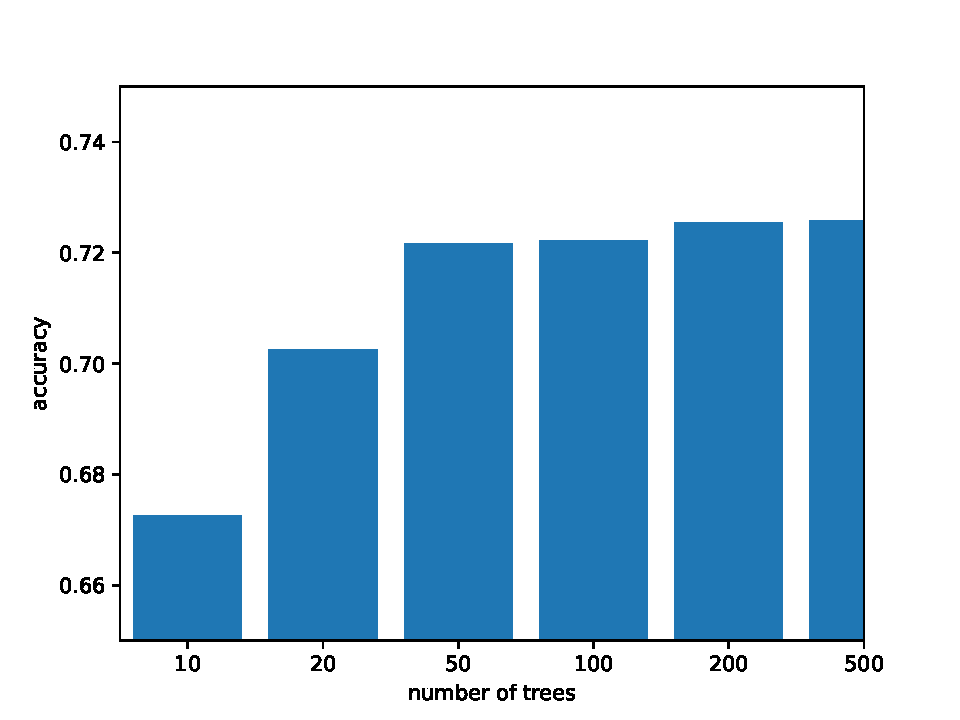
\includegraphics[scale=0.8]{images/trees.pdf}
    \caption{Graph showing the accuracy of the random forest model with different numbers of trees.}
    \label{fig:trees}
\end{figure}

Our random forest performed worse on the original data set,
achieving an accuracy of 71.78\%. None of the other parameters we changed helped the forest's predictive ability significantly, and changing them often led to worse results.
The parameter that was closest to being relevant was the max features parameter; we ultimately used sci-kit learn's default, which used the square root of the total features, to
achieve our best result. The closest we were able to get while changing the parameter was when we considered 10\% of the features, which increased our accuracy slightly with smaller sets of trees, but decreased performance when the number of trees was greater than 100; with 500 trees, it reached an accuracy of only 70.6\%. Our best results with the random forest model put us at a ranking of about 1028/1388 in the Kaggle competition.


%-Neural net results
%-using sci-kit learn's label encoder with keras.util's to_categorical allowed us to successfully transform our labels to something the neural net could understand
%-using more dense layers with relu activations was generally more successful
%-because of the number of features, the model was very prone to overfitting, and we increased the dropout rate between layers as much as we could before the results were worse

%adagrad and adam both generally performed better then sgd
%improvement with more epochs
\begin{figure}
    \centering
    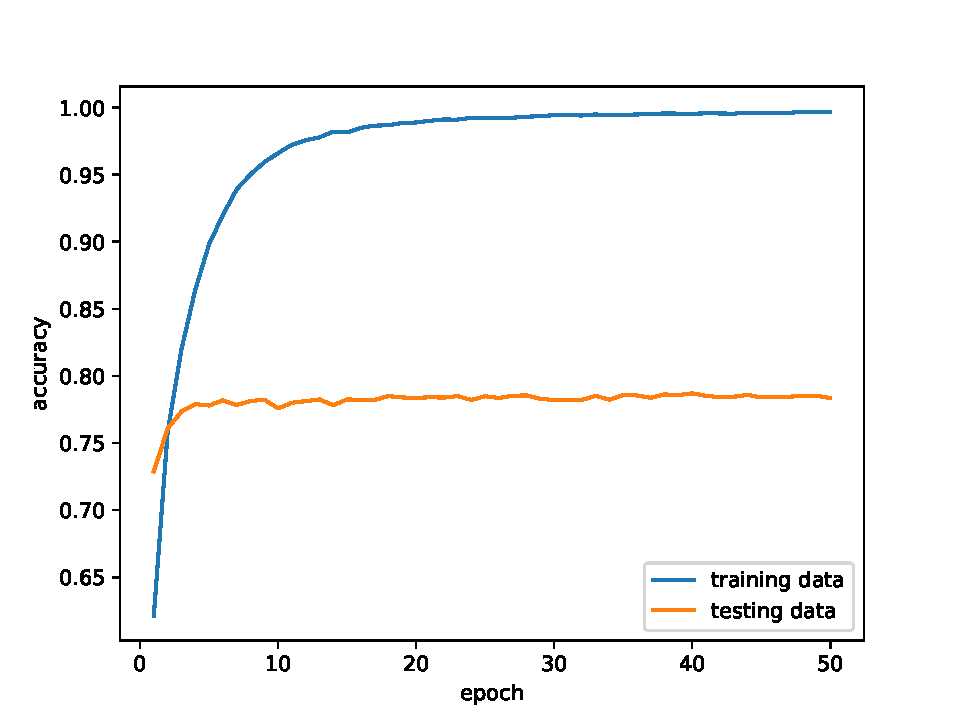
\includegraphics[scale=0.8]{images/epochs.pdf}
    \caption{Graph showing testing accuracy and training accuracy for the neural network. The large difference between the two lines indicates extreme overfitting.}
    \label{fig:epochs}
\end{figure}
\subsection{Neural Network Model}
For the neural network, the highest predictive accuracy we achieved with the cleaned data set was 78.35\%. This neural network had 5 dense layers, with 1024, 512, 256, 128, and 20 units from the
input later to the output layer. All these layers used the ReLU activation function, with the exception of the output layer which used the softmax activation function.
Between each dense layer was a dropout layer with a dropout rate of 0.4. The loss function was categorical cross-entropy and the optimizer was Adagrad; Adam had slightly worse
performance with a peak accuracy of 77.6\%, while stochastic gradient descent was slightly worse still with a peak accuracy of 75.35\%. We trained our
network for 50 epochs. Notably, while the predictive accuracy on the test set increased slowly and eventually leveled out during the 50 epochs, our neural network
started to overfit extremely very quickly, eventually reaching accuracies of 99\% on the training data during epochs, as
shown in Figure \ref{fig:epochs}. We increased the dropout rates as much as we could, and found
that after a rate of 0.4 the accuracy on the test set dropped; for example, the same network with dropout rates of 0.5 had an accuracy of 77.85\% and a minimal decrease
in overfitting. With the original data, the same neural net achieved an accuracy of 78.16\%. Our best neural network's results put us at a ranking of about 641/1388 in the Kaggle competition.


%-effectiveness of cleaning data:
%-random forest-> improvement
%-neural net -> improvement up until a certain point


%%%%%PLOT IDEAS%%%%%%%%%%
%Random forest: with other paramaters constant, change in accuracy as number of trees increased
                %change in accuracy as max features changed?

%Neural Net: improvement as more dense layers added?
            %improvement with changing dropout?

%Both: bar graph showing difference between best results with cleaned and uncleaned data?


\section{Conclusions}
\subsection{Discussion of Findings}
%This section should sum up what you did and what you found.
Given a large set of recipes and the cuisine categories they belonged to, we aimed to build 2 models for predicting the cuisine types of a test set of recipes.
By using one-hot encoding, we were able to vectorize our complex, non-numerical input set and make it usable for both the random forest and the neural network. We cleaned
the original data set to reduce the number of ingredients in recipes which were essentially the same but were counted as different features, and both of our models generally
predicted better as a result. Our data preprocessing produced a larger increase in accuracy in the random forest model than in the neural network model.

The best accuracy of our random forest model was 72.71\%, with cleaned data and 500 trees in the forest. This level of accuracy would likely not have been possible with a single decision tree, because the large number of features in our data set would be difficult to differentiate without extreme overfitting.

The neural network performed notably better than the random forest, with a best accuracy of 78.35\%. However, this was at the price of heavy overfitting; this is likely
due to the large number of features, the 6000+ ingredients. Changing the optimizer from stochastic gradient descent to Adagrad notably increased the accuracy, potentially because
Adagrad maintains different learning rates for each of its parameters unlike SGD and better captures the complexity and wide-range of our features as a result.

\subsection{Looking to the Future}
We believe that a higher accuracy could be achieved with better preprocessing of the data. Our ``cleaned" data set still contained a large number of redundant ingredients. Additionally, we could investigate using scikit-learn's DictVectorizer or some other feature extractor pre-training. Most of our data processing was done by hand, and there are almost certainly more sophisticated methods available. For the neural network, we could look into other ways to reduce the overfitting of our model without decreasing our
predictive accuracy in addition to adding dropout layers; given the large set of input features, this might also lie in finding some other way to succinctly vectorize our
data without losing the complex differences between recipes of different cuisines.


%With the random forest we found that the tradeoff in runtime when adding more decision trees was generally worth it; with a dataset with as many features as ours there are
%many possible variances between what trees predict from the different bootstrapped samples, so having more to average out/vote amongst was worth it
%it wasn't as clear how helpful refining the number of features was, but 0.1 was generally a sweet spot because we didn't drop out as many features as sqrt but still
%tried to account for a significant amount. the tradeoff in runtime was generally worthwhile, but not beyond 0.1 where we sometimes saw worse results, perhaps due
%to overfitting as we try to account for too many features

%For the neural net, adam and adagrad performed better than sgd because...WHYYYYYYYYYYYYYY
%adagrad performed better than adam because WHYYYYYYYYYYYY
%categorical_cross_entropy was an ideal loss function because we have multiple categorical outputs

\end{document}
